\section{CTL (computation tree logic)}
This part of the exam is about CTL, computation tree logic. For convenience
we reproduce a 0-based CTL semantics here (as opposed to Huth+Ryan who use a
1-based notation.) Let ${\cal M} = (S,\imp,L)$ be a model. Recall that
$P_{\cal M}(s)$ is the set of paths in model ${\cal M}$ starting with state
$s$, and that $\sigma[i]$ is the $i$th element (state) of path $\sigma$
(0-indexed in the semantics below, 1-indexed in Huth+Ryan).

{\bf 0-based CTL semantics:}
\begin{align*}
	{\cal M}, s &\models \top \\
	{\cal M}, s &\not\models \bot \\
	{\cal M}, s &\models p \qquad\Leftrightarrow\qquad p \in L(s) \\
	{\cal M}, s &\models \neg\phi \qquad\Leftrightarrow\qquad
		{\cal M}, s \not\models \phi \\
	{\cal M}, s &\models \phi_1 \land \phi_2 \qquad\Leftrightarrow\qquad
		{\cal M}, s \models \phi_1 \land {\cal M}, s \models \phi_2 \\
	&\vdots
\end{align*}
You may use either the 0-based or 1-based semantics to answer this part of the
exam, but be sure to clearly mark which one you use in your answer.

\subsection*{Question 5.3 \mdseries The Boolean function $g$ of 4 arguments
is defined by \[g(p,q,p',q') = p \cdot \overline{q'} + \overline{p} \cdot q'\]
where we follow the notation from representation of transistion functions from
symbolic model checking, such that $x'$ (where $x$ is an atom) denotes the
value of the next state.}
\subsubsection*{(a) \mdseries Construct a model ${\cal M}_g =
(S_g, \imp_g, L_g)$ such that $g$ represents the transition relation $\imp_g$
of the model. You may assume that the set of atomic propositions is ${p, q}$,
thus your model should have 4 states.}

\usetikzlibrary{arrows,positioning}
\begin{figure}[H]
	\center
	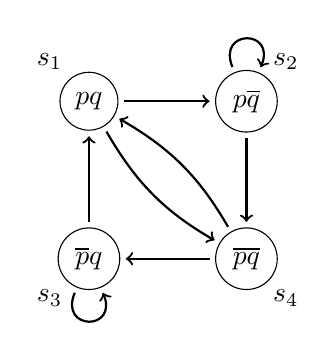
\begin{tikzpicture}
	[
	align=center,
	node/.style={circle,draw=black,fill=none},
	label/.style={draw=none,fill=none},
	arrow/.style={
           ->,
           thick,
           shorten <=2pt,
           shorten >=2pt,}
	]
		% nodes
		\node[node] (n1) at 		(-1.0,  1.0 ) {$p q$};
		\node[node] (n2) at 		( 1.0,  1.0 ) {$p \overline q$};
		\node[node] (n3) at 		(-1.0, -1.0 ) {$\overline p q$};
		\node[node] (n4) at 		( 1.0, -1.0 ) {$\overline p \overline q$};
		
		% labels
		\node[label] (l1) at 		(-1.5,  1.5 ) {$s_1$};
		\node[label] (l2) at 		( 1.5,  1.5 ) {$s_2$};
		\node[label] (l3) at 		(-1.5, -1.5 ) {$s_3$};
		\node[label] (l4) at 		( 1.5, -1.5 ) {$s_4$};
		
		% straight paths
		\foreach \from/\to in {n1/n2,n2/n4,n4/n3,n3/n1} \draw[arrow] (\from) -> (\to);
		
		% curved paths
		\draw[arrow] (n1) to [out=300,in=150,looseness=1] (n4);
		\draw[arrow] (n4) to [out=120,in=330,looseness=1] (n1);
		\draw[arrow] (n2) to [out=112.5,in=67.5,looseness=5] (n2);
		\draw[arrow] (n3) to [out=247.5,in=292.5,looseness=5] (n3);
		
	\end{tikzpicture}
	\label{fig:M_g-model}
	\caption{Model of ${\cal M}_g$}
\end{figure}

\newpage
\subsubsection*{(b) \mdseries Implement the model ${\cal M}_g$ in NuSMV with
all states as starting state. You may either use the 'stateful' or 'stateless'
approach (see first lecture on NuSMV).}
The code below translates all possibilities of movement along the paths of the
model ${\cal M}_g$ given.\footnote{Included with submission, see file
{\tt 5\_3b.smv} archived in {\tt code.zip}}
\begin{figure}[H]
	\lstinputlisting{M_g.smv}
	\label{code:M_g}
	\caption{NuSMV code of the ${\cal M}_g$ model}
\end{figure}
